% 8 pages + 2 pages of refs

\documentclass[11pt]{article}

%\usepackage{naaclhlt2013}
\usepackage{acl2013}
\usepackage{graphicx}
\usepackage{algorithmic}
\usepackage{times}
\usepackage{latexsym}
\usepackage{multirow}
\usepackage{url}
\usepackage{subfigure}
\usepackage{array}
\usepackage{sparklines}
\usepackage{amsmath,amsfonts,amssymb,amsthm}



\usepackage{paralist}
\usepackage{color}
%\usepackage{setspace}



\renewcommand{\baselinestretch}{0.98}
%\let\env=\texttt
%\let\pkg=\textsf
%\definecolor{sparkrectanglecolor}{rgb}{0.8,0.95,0.8}
%\definecolor{sparkspikecolor}{rgb}{1,0,0}
%\setlength{\sparkdotwidth}{1.3pt}
%\setlength{\sparklinethickness}{.3pt}

\DeclareMathOperator*{\argmax}{arg\,max}
  %\setlength\titlebox{6.5cm}    % Expanding the titlebox

\newcommand{\comment}[1]{} 
\newcommand{\NOTE}[1]{\marginpar{\em {#1}}}
\newcommand{\bug}
    {\mbox{\rule{2mm}{2mm}}}
\newcommand{\Bug}[1]
    {\bug \footnote{BUG: {#1}}}
\newcommand{\QED}{\mbox{$\Box$}}
\newcommand{\ddt}{\mbox{$\frac{d}{dt}\,$}}  %* no strut

\newcommand{\etal}{\mbox{\it et al.}}
\newcommand{\etc}{\mbox{\it etc.}}
\newcommand{\eg}{\mbox{\it e.g.}}
\newcommand{\ie}{\mbox{\it i.e.}}
\newcommand{\cf}{\mbox{\it cf.}}
\newcommand{\Eg}{\mbox{\it E.g.}}
\newcommand{\Ie}{\mbox{\it I.e.}}
\newcommand{\?}{\mbox{?}}




\newcommand{\DEFN}{\mbox{$\stackrel{\mbox{\tiny def}}{=}$}}

\newcommand{\TT}[1]{\mbox{\tt #1}}
%\newcommand{\bi}{\begin{itemize}}
%\newcommand{\ei}{\end{itemize}}
\newcommand{\bi}{\begin{list}{$\bullet$}{
    \setlength{\leftmargin}{1.5 em}
    \setlength{\itemsep}{0 pt}
    \setlength{\topsep}{3 pt}
    \setlength{\parsep}{3 pt}
    \setlength{\partopsep}{0 pt}
    \setlength{\labelwidth}{1 em}
    \setlength{\labelsep}{0.5 em}
    \setlength{\parskip}{0cm}  }}
\newcommand{\ei}{\end{list}}

\newcommand{\BE}{\begin{enumerate}}
\newcommand{\EE}{\end{enumerate}}

%\newtheorem{defnctr}{Definition}
%\newtheorem{theorem}{Theorem}
%\newtheorem{lemma}[theorem]{Lemma}
%\newtheorem{corollary}[theorem]{Corollary}        
%\newtheorem{conjecture}[theorem]{Conjecture}
%\newtheorem{propos}[theorem]{Proposition}
%\newcommand{\proof}
%	{\vspace{-8pt}
%	 {\bf Proof:}}



\newcommand{\tuple}[1]
        {\mbox{$\langle{#1}\rangle$}}
\newcommand{\set}[1]
        {\mbox{$\{{#1}\}$}}
\newcommand{\size}[1]{\mbox{$\mid\!#1\!\mid$}}



\newcommand{\PROOF}[1]{\mbox{\noindent \proofbegin {#1} \proofend}}
\newcommand{\proofbegin}{\mbox{\bf Proof: \ }}
\newcommand{\proofend}{\Math{\Box}}
\newcommand{\st}{\mbox{ such that }}
\newcommand{\wht}{\mbox{ we have that }}
\newcommand{\entails}{\mbox{$\models$}}
\newcommand{\yields}{\mbox{$\models$}}
\newcommand{\dgets}{\mbox{$\leftarrow$}}

%\renewcommand{\baselinestretch}{0.985}




\newcommand{\initab}{                           % set up tab stops
\begin{tabbing}
XXX \= XXXX \= \kill
}
\newcommand{\begpub}{
\begin{quotation}
\noindent
}
\newcommand{\nextpub}{

\vspace{2mm}
\noindent
}
\newcommand{\finpub}{
\end{quotation}
}



\hyphenation{non-de-ter-mi-nis-tic-al-ly non-de-ter-mi-nis-tic
exis-ten-tial-ly quan-tified se-lec-tion exis-ting in-stan-tiated
uni-vers-al-ly es-tab-lish in-con-sis-tent}


% \newcommand{\ncd}{\mbox{$\neq$}}
% \newcommand{\cd}{\mbox{$=$}}
% \newcommand{\fabian}{\mbox{\sc fabian}}
% \newcommand{\occam}{\mbox{\sc occam}}
% \newcommand{\sadl}{\mbox{\sc sadl}}
% \newcommand{\socrates}{\mbox{\sc socrates}}
% \newcommand{\uwl}{\mbox{\sc uwl}}
% \newcommand{\spa}{\mbox{\sc spa}}
% \newcommand{\scr}{\mbox{\sc scr}}
% \newcommand{\strips}{\mbox{\sc strips}}
% \newcommand{\snlp}{\mbox{\sc snlp}}
% \newcommand{\cbur}{\mbox{\sc C-buridan}}
% \newcommand{\buridan}{\mbox{\sc buridan}}
% \newcommand{\xii}{\mbox{\sc xii}}
% \newcommand{\zeno}{\mbox{\sc zeno}}
% \newcommand{\adl}{\mbox{\sc adl}}
% \newcommand{\kr}{\mbox{\tt /kr94}}
% \newcommand{\ucpop}{\mbox{\sc ucpop}}
% 
% \newcommand{\cause}{{\tt cause}}
% \newcommand{\observe}{{\tt observe}}
% \newcommand{\satisfy}{{\tt satisfy}}
% \newcommand{\handsoff}{{\tt hands-off}}
% \newcommand{\findout}{{\tt find-out}}
% 
% \newcommand{\CAUS}{\mbox{C}}
% \newcommand{\OBS}{\mbox{O}}
% \newcommand{\PAT}{\mbox{\sf E}}
% \newcommand{\fact}{\mbox{$\varphi$}}
% \newcommand{\LIT}{\mbox{\sf p}}
% \newcommand{\lit}{\mbox{\LIT}}
% \newcommand{\litp}{\mbox{\LIT$^\prime$}}
% \newcommand{\rel}{\mbox{REL}}
% \newcommand{\change}[3]{\mbox{$\Delta(#1,{\tt #2}\rightarrow {\tt #3})$}}   
% 
% \newcommand{\true}{{\tt T}}
% \newcommand{\false}{{\tt F}}
% \newcommand{\unknown}{{\tt U}}
% 
% 


\def\upcase{\expandafter\makeupcase}



\newcommand{\hrone}{temporal functionality heuristic}
\newcommand{\hrtwo}{temporal burstiness heuristic}
\newcommand{\hrthree}{one event-mention per discourse heuristic}
\newcommand{\hrfour}{Tense Consistency Heuristic}


\newcommand{\temporal}{Temporal Hypotheses}
\newcommand{\sys}{\mbox{\sc CrowdAnno}}   % afar
\newcommand{\kylin}{\mbox{\sc Kylin}}
\newcommand{\tr}{\mbox{\sc TextRunner}}
\newcommand{\E}{\mbox{$\mathbf e$}}

%\newcommand{\mtt}[1]{\mbox{$\tt{#1}$}}
\newcommand{\bmtt}[1]{\mbox{$\tt{\mathbf{#1}}$}}

\newcommand{\eat}[1]{}

\newcommand{\Eec}{\mbox{\em extracted event candidate}}
%\newcommand{\Eec}{Extracted Event Candidate}
%\newcommand{\Eec}{\mbox{Extracted Event Candidate}}
\newcommand{\eec}{\mbox{EEC}}
\newcommand{\bag}{\mbox{EEC-set}}

\newcommand{\mtt}[1]{{\it #1}}


\title{Visualizing NLP annotations for Crowdsourcing }

%\title{Distant Supervision for Information Extraction of Polymorphic Tuples}
%\title{Distant Supervision for Information Extraction
%                   without Relational Exlcusivity}


\author{Hanchuan Li, Haichen Shen, Shengliang Xu and Congle Zhang\\
 Computer Science \& Engineering \\
 University of Washington\\
 Seattle, WA 98195, USA \\
 {\tt \{hanchuan,haichen,shengliang,clzhang\}@cs.washington.edu} \\}


%\date{}




\begin{document}

\maketitle

\begin{abstract}
Visualizing NLP annotation is useful for the collection of training data for the statistical NLP approaches.  Existing toolkits either provide limited visual aid, or introduce comprehensive operators to realize sophisticated linguistic rules. Workers must be well trained to use them. Their audience thus can hardly be scaled to large amounts of non-expert crowd-sourced workers. In this paper, we present \sys, a visualization toolkit to allow crowd-sourced workers to annotate two general categories of NLP problems: clustering and parsing. Workers can finish the tasks with simplified operators in an interactive interface, and fix errors conveniently. User studies show our toolkit is very friendly to NLP non-experts, and allow them to produce high quality labels for several sophisticated problems. We release our source code and toolkit to spur future research.
\end{abstract}


\section{Introduction}

With the popularity of the Intenet, there are huge amount of text in the web, and their size is still growing quickly. In order to use them, it is of utmost importance to develop automatic nature language processing (NLP) systems to handle the big data. 

%A typical NLP system would first employ syntactic processing and then employ semantic processing.  Syntactic processing is often task independent. It aims to convert the raw text into some machine friendly structures. The pipeline often includes tokenization, POS tagging, parsing, name entity recognition and coreference. Semantic processing is often task dependent. It tries to exploit useful information from the text for an end  task. 

It has been wildly accepted that statistical machine learning approaches are very effective for most NLP problems, such as parsing~\cite{klein2003accurate}, information extractions~\cite{banko2007open}, question answering~\cite{kwok2001scaling} and so on. However, there is a significant limitation of all the statistical approaches: they need a lot of training data to learn the model. These training data are labeled by annotators. In most cases, annotators manually predict the desired outputs for the inputs. The algorithms then learn the statistics and models from the training data and use them to automatically predict the output of the unlabeled data.   

Generally, labeling datasets for machine learning problems (often classification) is time consuming and tedious. To make matters worse, it is even harder for annotators to label NLP problems than to label standard classification problems. For a standard classification problem, human annotators are given a set of labels and a list of objects. Their jobs are to choose a label for each object. Since objects are usually independent of each other, the prediction is local and straightforward. Besides, labeling errors, if any, would not affect the rest of the dataset. Therefore, the user interface for the annotations could be very naive: plain text or Excel tables are often enough in many cases. 


But for NLP annotations, the outputs are often structured predictions. That is, each prediction is depending on some other prediction. For example, Figure 1 shows how parsing algorithm converts a sentence into a tree. It is hard for annotators to decide the position of a single word in the tree before drawing the whole tree. Besides, a large group of NLP problems are related to clustering, such as coreference resolution~\cite{lee2011stanford}, which clusters two or more expressions in a text refer to the same person or thing. Unlike classification, annotates must acquire some global information before correctly labeling the clusters. Suppose there are ``Jeffery Heer", ``Jeff Bilmes", ``Jeff", ``the professor" in a text. To decide whether which ``Jeff" and which ``professor", annotator must read the context to know who they are. Transitivity also makes the clustering annotation very tricky. For example, after merging some pairs of points, the annotator has created two clusters $\{$``Jeff, Jeff Bilmes''$\}$ and $\{$``Jeffery Heer, Professor Heer''$\}$. He then accidentally merges ``Jeff" and ``Jeffery Heer".  It would immediately result in a very large and incorrect cluster.


The challenges listed above makes the labeling process uncomfortable for normal annotators. Firstly, annotators must spend a lot of time to understand the global structure of the data before labeling anything. Secondly, annotators would often revisit and edit their labels. In the above example, the annotator notices that ``Jeff Bilmes" and ``Jeffery Heer" are in the same cluster, then he has to go back and fix that error. Such trial and errors could cause conflicts and incomplete annotations. In fact, even trained linguistic must spend a lot of time to label NLP datasets. A famous example is that it costs 8 years to create the Penn Tree Bank, a labeled dataset of parsed trees. 

Nowadays, there are many worker at crowdsourcing platforms like Mechanical Turks\footnote{~\url{https://www.mturk.com/mturk/welcome}} and Odesk. They provide us opportunities to quickly collect a large amount of training data. But most workers are normal people, having little knowledge about linguistic, and having no reason to be patient enough. If the problem is to hard, they would switch to other easier and profitable jobs. So it is impractical to ask them to label over plain text files or Excel tables for NLP annotations.  
\section{Toolkit Overview}
In this section, we first introduce the design decisions and the overview of the toolkits. Then we present the user interface and the major functions.

Firstly, the toolkit is designed and implemented as a web application, since it is easiest for crowd workers to visit.

The users of our visualization toolkit include {\em annotation gatherers} and {\em crowd-source workers}. In general, annotation gatherers use our toolkit to collect training data from crowd-source workers for their NLP systems. It is reasonable to assume they are NLP experts and well-trained programmers. We believe annotation gatherers know their NLP problems better than anyone else, so we leave them to implement the visualization of the NLP task by implementing a static page. They should embed the APIs of our toolkits in their html so they can pass on the objects to cluster or parse. We keep the task-visualization transparent to maximize the flexibility of our toolkit. Figure~\ref{fig:workflow} shows the workflow of our toolkit.

\begin{figure}
\centering
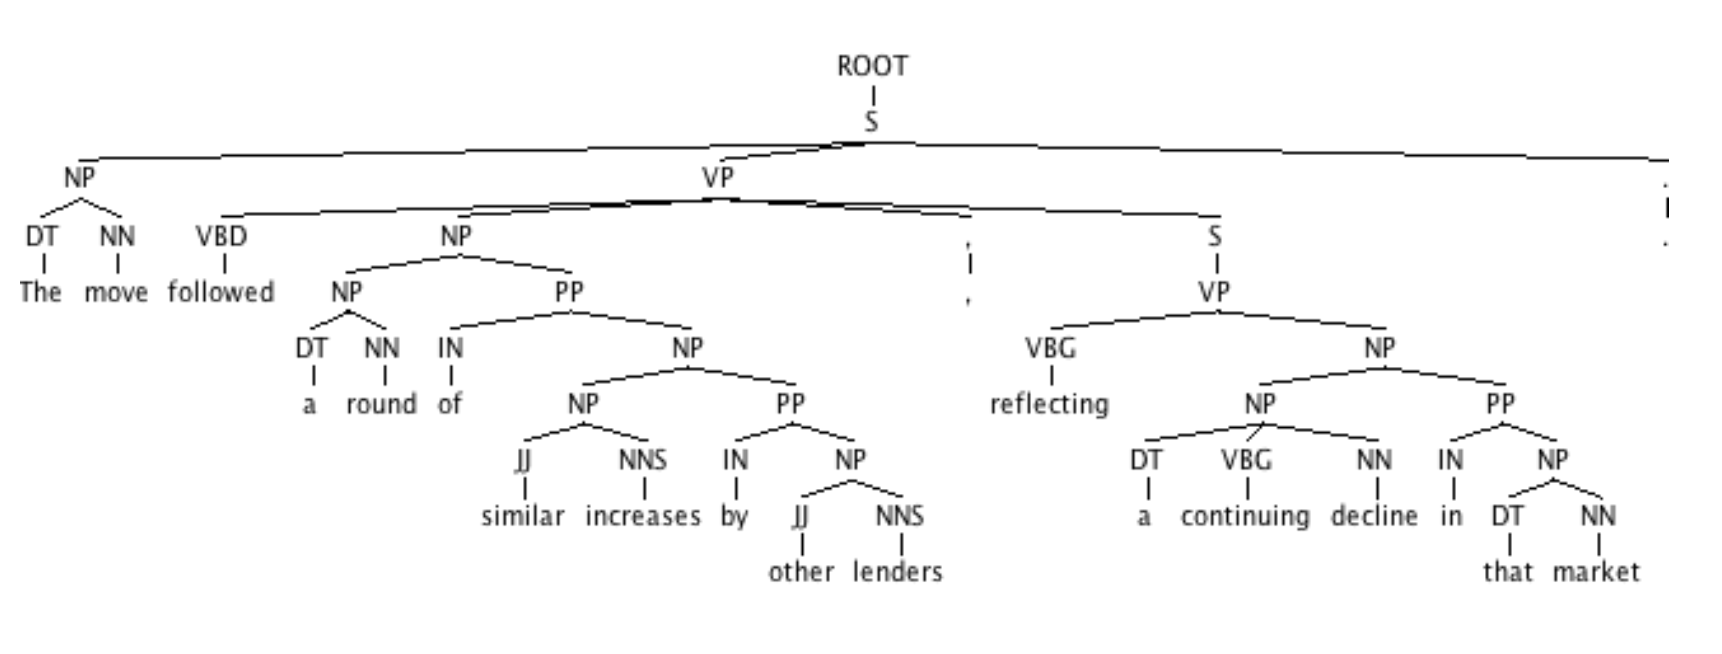
\includegraphics[width=3.1in]{figs/parsetree.png}
\caption{An example parse tree.}
\label{fig:workflow}
\end{figure}



In this project, we aim to develop a visualized toolkit for
crowd-sourcing NLP annotations. The target audience are normal people
with little knowledge and patience. The toolkit would allow them to
quickly label NLP datasets.

There are two key properties of our toolkit: firstly, annotators could
interact with the data to understand them in a refresh way. Annotators
label some examples and they expect immediate feedback from the
toolkit. These feedbacks will help them understand the problem.
Secondly, the toolkit should enable and encourage trial and errors. It
would not assume any edits from the users as gold, but treat the edits
as clues to better visualize the data to the annotator. When the
annotator finishes a labeling task, he should be satisfied and
confident with the overall outcome. For example, it is hard to
distinguish whether ``Jeff" is ``Jeff Bilmes" or ``Jeffery Heer" when
data points are seen individually. But if the toolkit could immediate
show a big cluster $\{$``Jeff, Jeff Bilmes, Jeffery Heer, Professor
Heer"$\}$ after incorrectly merge two points, the annotators would
have a good chance to fix it.

In this project, we would focus on two important kinds of NLP
annotations: building trees (\eg\  parsing) and clustering (\eg\
coreference resolution). But we would keep in mind that the toolkit
should be easily extensible to any NLP problems.

\subsection{Building tree}

Formally, the input is a list of nodes, the output would be a tag for
each node. Nodes sharing the same tag stay in the same cluster. Let us
use the following running example: the task is to co-refer five
mentions ``Jeffery Heer", ``Jeff Bilmes", ``Jeff", ``Professor Heer"
and ``Mr Bilmes". We propose to use ``dependency wheel" for this task.
At first, annotator would see 5 objects listed on the right side of
the window, and there is nothing on the wheel. He could operate the
data in the following ways:

Drag node $a$ to node $b$ when they are in the same cluster: suppose
we drag ``Jeff" to ``Jeffery Heer". They would be added to the wheel
if not yet. Suppose ``Jeff'', ``Jeffery Heer'' are in clusters
  $\{$``Jeff, Jeff Bilmes''$\}$ and $\{$``Jeffery Heer, Professor
  Heer''$\}$. Then the resulting cluster would be $\{$``Jeff, Jeff
  Bilmes, Jeffery Heer, Professor Heer"$\}$. All four nodes will be
  colored the same and group together on the wheel. There is also an
  ``yes" edge between ``Jeff'' and ``Jeffery Heer'' highlighting this
  operator.

Two nodes are different: annotators soon notice that ``Jeff Bilmes"
and ``Jeffery Heer" in the resulting cluster is bad. But he is not
aware of which previous edit causes this error. So he just tell the
toolkit that ``Jeff Bilmes" and ``Jeffery Heer" are two different
entities. There comes a ``no" edge between them. The system would
figure out this different edge is conflict with the previous ``yes"
edge between ``Jeff'' and ``Jeffery Heer''. The toolkit would
highlight the conflicts so annotator could cancel one or several of
them.

Tag the nodes: nodes with the same tag would be grouped together and
put together on the wheel. The tag could cause conflicts. The toolkit
would automatically figure them out and highlight them on the screen.
So annotators could easily trial and errors.


\subsection{Tree Generation}

Formally, the input is a list of nodes, the output would be a tree
whose leaf nodes are the input nodes. Besides, breadth-first search
the tree will not change the initial order of the nodes. Let us parse
the sentence ``My little dog also likes eating sausage." as a running
example. At first, annotators would see 6 individual nodes. He could
operate the tree in the following ways:

Drag node $A$ to node $B$ when they are siblings: if two nodes have no
parent node yet, we would create an inner node as the parent of the
two children, and add tree edges. For example, user can drag ``little"
to ``dog" to create a node for phrase ``little dog". If $B$ has its
parent $C$ already, $A$ will be linked to $C$ as its new child. For
example, user can drag ``My" to ``little" or ``dog" to merge ``my"
with ``little dog". This operator is enough to build the tree.

Click the edge to cancel parent-child relationship: when the parent
node loses all its children, the inner node will be removed from the
tree. This operator enables trial and error for annotators.

Tag the nodes: when linguistics build the parse tree, they would also
tag the POS tags (\ie\ verb, noun phrase). Since there are dozens tags
on the tree, it is too complicated for normal people to tag all of
them. But fortunately, a partial set of tags, especially verb and
nouns, would help the machine learning algorithms a lot. Annotators
could choose to tag some nodes with those most important tags. We
would also support edit and delete the tags.




%\section{Toolkit Overview}
In this section, we first introduce the design decisions and the overview of the toolkits. Then we present the user interface and the major functions.

Firstly, the toolkit is designed and implemented as a web application, since it is easiest for crowd workers to visit.

The users of our visualization toolkit include {\em annotation gatherers} and {\em crowd-source workers}. In general, annotation gatherers use our toolkit to collect training data from crowd-source workers for their NLP systems. It is reasonable to assume they are NLP experts and well-trained programmers. We believe annotation gatherers know their NLP problems better than anyone else, so we leave them to implement the visualization of the NLP task by implementing a static page. They should embed the APIs of our toolkits in their html so they can pass on the objects to cluster or parse. We keep the task-visualization transparent to maximize the flexibility of our toolkit. Figure~\ref{fig:workflow} shows the workflow of our toolkit.

\begin{figure}
\centering
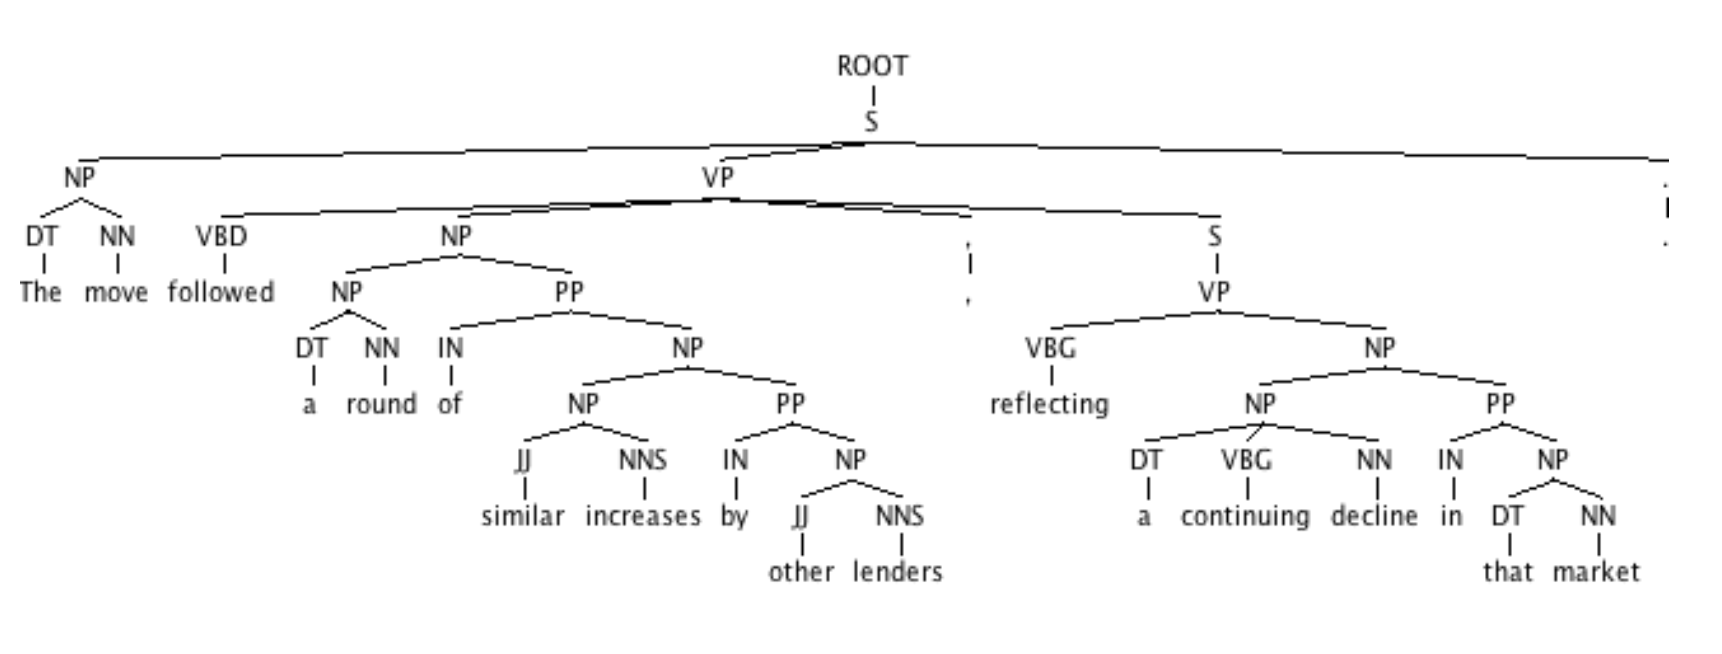
\includegraphics[width=3.1in]{figs/parsetree.png}
\caption{An example parse tree.}
\label{fig:workflow}
\end{figure}



In this project, we aim to develop a visualized toolkit for
crowd-sourcing NLP annotations. The target audience are normal people
with little knowledge and patience. The toolkit would allow them to
quickly label NLP datasets.

There are two key properties of our toolkit: firstly, annotators could
interact with the data to understand them in a refresh way. Annotators
label some examples and they expect immediate feedback from the
toolkit. These feedbacks will help them understand the problem.
Secondly, the toolkit should enable and encourage trial and errors. It
would not assume any edits from the users as gold, but treat the edits
as clues to better visualize the data to the annotator. When the
annotator finishes a labeling task, he should be satisfied and
confident with the overall outcome. For example, it is hard to
distinguish whether ``Jeff" is ``Jeff Bilmes" or ``Jeffery Heer" when
data points are seen individually. But if the toolkit could immediate
show a big cluster $\{$``Jeff, Jeff Bilmes, Jeffery Heer, Professor
Heer"$\}$ after incorrectly merge two points, the annotators would
have a good chance to fix it.

In this project, we would focus on two important kinds of NLP
annotations: building trees (\eg\  parsing) and clustering (\eg\
coreference resolution). But we would keep in mind that the toolkit
should be easily extensible to any NLP problems.

\subsection{Building tree}

Formally, the input is a list of nodes, the output would be a tag for
each node. Nodes sharing the same tag stay in the same cluster. Let us
use the following running example: the task is to co-refer five
mentions ``Jeffery Heer", ``Jeff Bilmes", ``Jeff", ``Professor Heer"
and ``Mr Bilmes". We propose to use ``dependency wheel" for this task.
At first, annotator would see 5 objects listed on the right side of
the window, and there is nothing on the wheel. He could operate the
data in the following ways:

Drag node $a$ to node $b$ when they are in the same cluster: suppose
we drag ``Jeff" to ``Jeffery Heer". They would be added to the wheel
if not yet. Suppose ``Jeff'', ``Jeffery Heer'' are in clusters
  $\{$``Jeff, Jeff Bilmes''$\}$ and $\{$``Jeffery Heer, Professor
  Heer''$\}$. Then the resulting cluster would be $\{$``Jeff, Jeff
  Bilmes, Jeffery Heer, Professor Heer"$\}$. All four nodes will be
  colored the same and group together on the wheel. There is also an
  ``yes" edge between ``Jeff'' and ``Jeffery Heer'' highlighting this
  operator.

Two nodes are different: annotators soon notice that ``Jeff Bilmes"
and ``Jeffery Heer" in the resulting cluster is bad. But he is not
aware of which previous edit causes this error. So he just tell the
toolkit that ``Jeff Bilmes" and ``Jeffery Heer" are two different
entities. There comes a ``no" edge between them. The system would
figure out this different edge is conflict with the previous ``yes"
edge between ``Jeff'' and ``Jeffery Heer''. The toolkit would
highlight the conflicts so annotator could cancel one or several of
them.

Tag the nodes: nodes with the same tag would be grouped together and
put together on the wheel. The tag could cause conflicts. The toolkit
would automatically figure them out and highlight them on the screen.
So annotators could easily trial and errors.


\subsection{Tree Generation}

Formally, the input is a list of nodes, the output would be a tree
whose leaf nodes are the input nodes. Besides, breadth-first search
the tree will not change the initial order of the nodes. Let us parse
the sentence ``My little dog also likes eating sausage." as a running
example. At first, annotators would see 6 individual nodes. He could
operate the tree in the following ways:

Drag node $A$ to node $B$ when they are siblings: if two nodes have no
parent node yet, we would create an inner node as the parent of the
two children, and add tree edges. For example, user can drag ``little"
to ``dog" to create a node for phrase ``little dog". If $B$ has its
parent $C$ already, $A$ will be linked to $C$ as its new child. For
example, user can drag ``My" to ``little" or ``dog" to merge ``my"
with ``little dog". This operator is enough to build the tree.

Click the edge to cancel parent-child relationship: when the parent
node loses all its children, the inner node will be removed from the
tree. This operator enables trial and error for annotators.

Tag the nodes: when linguistics build the parse tree, they would also
tag the POS tags (\ie\ verb, noun phrase). Since there are dozens tags
on the tree, it is too complicated for normal people to tag all of
them. But fortunately, a partial set of tags, especially verb and
nouns, would help the machine learning algorithms a lot. Annotators
could choose to tag some nodes with those most important tags. We
would also support edit and delete the tags.




%Evaluation of the system:

We will have separate evaluations of the two proposed visualization tools we will build for tow different tasks of natural language processing.

Clustering visualization
In order to evaluate the clustering visualization tool, we will compare that to a traditional linguistics  process of doing word clustering, where the participants are required to manually label each word according to different categories on a Microsoft Excel or similar chart software.

Participants: We will gather 10 native speaker participants form undergraduate/graduate CSE students.
Experiment: We will divide them into two groups, Each group will complete two standard linguistic clustering tasks with similar work load and difficulty. One of the group will conduct the task with help of our visualization tool first, the other will do the task without visualization first. Then the tow groups switch task.

Evaluation: Both time consumption and accuracy of the two groups of participants will be evaluated.

2. Tree Parsing

Because of the difficulty of the Tree Parsing tasks, there is actually no reliable way for people to conduct such tree parsing without tedious training. So our evaluation aim to discover how this good this tool can actually turn something almost impossible to reality.

Participants: We will gather 10 native speaker participants form undergraduate/graduate CSE students.
Experiment: participants will complete two standard linguistic parcing tasks with similar work load and difficulty. One of the group will conduct the task with help of our visualization tool first, the other will do the task without visualization first. Then the two groups switch task.

Evaluation: Both time consumption and accuracy of the two groups of participants will be evaluated.

\section{Related Work}

The vast majority of paraphrasing work falls into two categories:
approaches based on the distributional hypothesis or those exploiting on
correspondences between parallel
corpora~\cite{androutsopoulos2009survey,madnani2010generating}.

{\bf Using Distribution Similarity:} Lin and
Pantel's~\shortcite{lin2001discovery} DIRT employ mutual information
statistics to compute the similarity between relations represented in
dependency paths.  Resolver~\cite{yates2009unsupervised} introduces a
new similarity metric called the Extracted Shared Property (ESP) and
uses a probabilistic model to merge ESP with surface string
similarity.

Identifying the semantic equivalence of relation phrases is also 
called {\it relation discovery} or {\it unsupervised semantic
  parsing}.  Often techniques don't compute the similarity explicitly
but rely implicitly on the distributional hypothesis. Poon and
Domingos'~\shortcite{poon2009unsupervised} USP clusters relations
represented with fragments of dependency trees by repeatedly merging
relations having similar
context. Yao~\etal~\shortcite{yao2011structured,yaounsupervised}
introduces generative models for relation discovery using LDA-style
algorithm over a relation-feature matrix.
Chen~\etal~\shortcite{chen2011domain} focuses on domain-dependent
relation discovery, extending a generative model with meta-constraints
from lexical, syntactic and discourse regularities.

Our work solves a major problem with these approaches, avoiding errors
such as confusing synonyms with antonyms and causes with
effects. Furthermore, \sys\ doesn't require massive statistical
evidence as do most approaches based on the distributional hypothesis.



{\bf Using Parallel Corpora: } Comparable and parallel corpora,
including news streams and multiple translations of the same story,
have been used to generate paraphrases, both
sentential~\cite{barzilay2003learning,dolan2004unsupervised,shinyama2003paraphrase}
and
phrasal~\cite{barzilay2001extracting,shen2006adding,pang2003syntax}. Typical
methods first gather relevant articles and then pair sentences that
are potential paraphrases.  Given a training set of paraphrases,
models are learned and applied to unlabeled
pairs~\cite{dolan2005automatically,SocherEtAl2011:PoolRAE}. Phrasal
paraphrases are often obtained by running an alignment algorithm over
the paraphrased sentence pairs.

While prior work uses the temporal aspects of news streams as a coarse
filter, it largely relies on text metrics, such as context similarity and
edit distance, to make predictions and alignments. These metrics are
usually insufficient to produce high precision results; moreover they tend
to produce paraphrases that are simple lexical variants (\eg\ {\it \{go to,
go into\}.}). In contrast, \sys\ generates paraphrase clusters with both high
precision and high diversity.

{\bf Others:}
Textual entailment~\cite{dagan2009recognizing}, which finds a phrase
implying another phrase, is closely related to the paraphrasing task.
Berant~\etal~\shortcite{berant2011global} notes the flaws in distributional
similarity and proposes local entailment classifiers, which are able to combine
many features. Lin~\etal~\shortcite{lin2012no} also uses temporal information to
detect the semantics of entities. In a manner similar to our approach,
Recasens~\etal~\shortcite{recasens2013same} mines parallel news stories to find
opaque coreferent mentions.











%The source code of our system, its output, and all data annotations are available at {\tt http://cs.uw.edu/homes/raphaelh/mr}.
%
\bibliographystyle{naaclhlt2013}
\bibliography{general,proposal,progressreport}

\end{document}


